\section{Let Neural Nets learn high frequency content in low dimensional domain}

\begin{figure}[H]
    \centering
    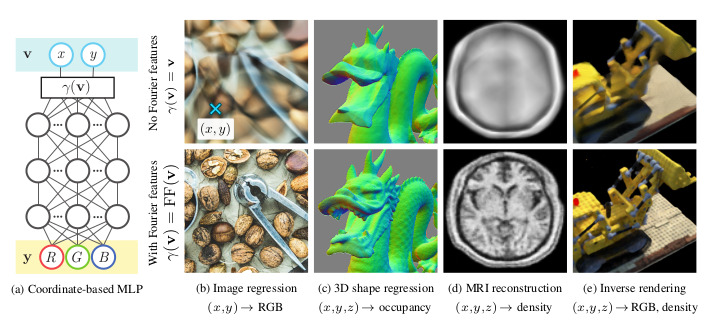
\includegraphics[width=\linewidth]{images/chapter3_img/fourierFeaturesInCoordinatesBasedMLP.jpg}
    \caption{Βελτίωση αποτελεσμάτων σε Coordinate Based MLPs για μια ποικιλία υψηλοσυχνοτικού περιεχομένου εφαρμοσμένο σε χαμηλοσυχνοτική εφαρμογή της ανακατασκευής εικόνων και 3D σχημάτων, Πηγή \cite{tancik2020fourier}}
    \label{fig:enter-label}
\end{figure}

Τα δίκτυα που ασχολούνται με την νευρωνική απόδοση όγκου καθώς και δίκτυα ανακατασκευής σημάτων ασχολήθηκαν σε βάθος με την κωδικοποίηση της εισόδου για την καταγραφή του συχνοτικού περιεχομένου που έχει η επιφάνεια και πρέπει να φανεί τόσο στην γεωμετρία της όσο και στις παραμέτρους που αναπαριστούν το χρώμα της κατά την απόδοση της σκηνής.

Αυτή η ιδέα παρουσιάζεται στο NeRF \cite{mildenhall2020nerf}, με την μορφή του \enit{Positional Encoding} το οποίο αναλύθηκε και στο \ref{section:dnnEmbeddings}. Ωστόσο, το βασικό θεωρητικό υπόβαθρο αυτής της τεχνικής, η οποία είναι σε θέση να βρει υψηλοσυχνοτικές σχέσεις δεδομένων αντιστοιχώντας τα με ειδικές συναρτήσεις πυρήνα Fourier σε υψηλότερες διαστάσεις όπου αναπαριστώνται καλύτερα χαρακτηριστικά (\enit{Hilbert Space}), διατυπώθηκε ξεκάθαρα στα πλαίσια της εργασίας \enit{Fourier Feature Networks / Let Neural Networks Learn High frequency content from low dimensional input} \cite{tancik2020fourier}. 

Συγκεκριμένα τα νευρωνικά δίκτυα προσπαθούν να προσεγγίσουν συναρτήσεις ρυθμίζοντας τις παραμέτρους των βαρών τους μέσω αλγορίθμων που βασίζονται στην πτωτική κλίση σφάλματος (\enit{Stochastic Gradient Descent} \cite{lecun2015deep}). Όταν ο στόχος είναι το μοντέλο να γενικεύει καλά στην διαδικασία προσέγγισης, τα δίκτυα είναι καταδικασμένα να ενσωματώσουν πολλές περισσότερες παραμέτρους για να μοντελοποιήσουν συναρτήσεις που δίνουν ακριβείς τιμές. Αυτό σε έναν βαθμό βελτιώνεται όταν προσπαθούμε να προσαρμόσουμε τα βάρη στα δεδομένα μέσω θεωρίας ομαλοποίησης βαρών. Έτσι θεωρείται ότι δίνονται βαθμοί ελευθερίας ώστε να μπορέσει το δίκτυο να δράσει καλύτερα εκτός του συνόλου εκπαίδευσης. Ωστόσο, μη επαρκής ομαλοποίηση οδηγεί το δίκτυο σε προβλήματα υπερεκπαίδευσης το οποίο θεωρείται ότι συνήθως μπορεί να ξεπεραστεί στα πλαίσια της δημιουργίας συνόλου δεδομένων υψηλής εντροπίας, και τεχνικών εκπαίδευσης όπως στρώματα \enit{Dropout} που τυχαία κόβουν υπολογιστικούς κόμβους, ή τεχνικές κανονικοποίησης / ομαλοποίησης που εμφανίζονται στα πλαίσια εκπαίδευσης (πχ.\enit{Batch Normalization}, δηλαδή κανονικοποίηση κατά ομάδες δεδομένων εκπαίδευσης που συνδυάζεται με μεθόδους εκπαίδευσης \enit{mini Batch} όχι \enit{online}). 

Παρ' όλα αυτά, στα πλαίσια της εργασίας τα δίκτυα είναι πλήρως συνδεδεμένα \enit{MLPs} συνταγμένων. Δηλαδή η διάσταση είναι αρκετά μικρή και η τυχαιότητα των δεδομένων δεν είναι προφανής. Συνεπώς στα πλαίσια των εργασιών που προαναφέρθηκαν γίνεται μια προσπάθεια, αντί να προσεγγιστεί το πεδίο $f(x,y,z;\theta)$  για παράδειγμα, που είναι το έμμεσο πεδίο απόστασης από την επιθυμητή επιφάνεια, να προσεγγιστεί το πεδίο $\gamma(v;\theta)$. Αυτό το πεδίο,  έχει κωδικοποιήσει την είσοδο μέσα από έναν εφαπτόμενο πυρήνα ημιτονειδών συναρτήσεων δηλαδή συναρτήσεων που ενσωματώνουν συχνοτικό περιεχόμενο. Το είδος των συναρτήσεων εξασφαλίζει ότι δεν χάνεται το  συχνοτικό περιεχόμενο των δεδομένων όταν περνούν από συστήματα που μπορεί να μην μπορούν να το αντιληφθούν επειδή είναι υψηλότερης διάστασης από τα ίδια τα δεδομένα. Τέτοιου είδους πρόβλημα αντιμετωπίζουν απο την φύση της εκπαίδευσής τους οι υπολογιστικοί γράφοι των \enit{DNNs}(βαθιών νευρωνικών δικτύων).  


\subsubsection{ΝeRF Positional Encoding}
Έτσι το NeRF \cite{mildenhall2020nerf}, προσπαθεί να καταγράψει υψηλοσυχνοτικές σχέσεις στην απόδοση χρώματος στην ογκομετρική απόδοση χώρου εφαρμόζοντας το \enit{Positional Encoding} στα δεδομένα μια πρακτική που δίνει προοπτική στα αποτελέσματα ανακατασκευής του πεδίου ακτινοβολίας αλλά και στην ταχύτητα σύγκλισης σε καλά επίπεδα σφάλματος.

\subsubsection{Σφαιρικές Αρμονικές | Spherical Harmonic Encoder} 
Τέλος η χρήση σφαιρικών αρμονικών είναι μια τεχνική που χρησιμοποιείται αποκλειστικά για την κωδικοποίηση των διανυσμάτων προσανατολισμού της κάμερας, καθώς μοντελοποιούν ανακλαστικές ιδιότητες που έχουν να κάνουν με πεδία ακτινοβολίας ωστόσο αντιστοιχούν σε παρόμοιες μορφές κωδικοποίησης και όλη η ιδέα προήλθε από την παρακάτω πηγή \cite{nuajSphericalHarmonicsPortalWakapon} μιας και οι σφαιρικές αρμονικές είναι κλασσική μέθοδος ανακατασκευής σήματος και προήλθε από έρευνα κβαντομηχανικής πάνω στο σωματίδιο του υδρογόνου H. Έτσι ερευνήθηκε και το μοντέλο κωδικοποίησης σφαιρικών αρμονικών που βασίζεται στον υπολογισμό των παραμέτρων $C$ στην εξίσωση πραγματικών σφαιρικών αρμονικών  \ref{eq:RealSphericalHarmonics}.

Σε κάθε περίπτωση η συνένωση HF(υψηλοσυχνοτικών) κωδικοποιημένων εισόδων μαζί με πραγματικών συντεταγμένων, επιτρέπει στα δίκτυα να προσεγγίσουν με πολύ μεγαλύτερη αξιοπιστία συναρτήσεις στο πρόβλημα της παλινδρόμησης συντεταγμένων, με αποτέλεσμα να αποτυπώσουν υψηλοσυχνοτικό περιεχόμενο στις αναπαραστάσεις σε λίγες εποχές εκπαίδευσης με λιγότερες παραμέτρους εκπαίδευσης.